\chapter{TINJAUAN PUSTAKA}
% contoh opsi lain Bab 2
%\chapter{DASAR TEORI}


%\section{Landasan Teori}
%\noindent Penelitian ini didasarkan pada beberapa landasan teori yang relevan dengan segmentasi mikrovaskular ginjal menggunakan model \textit{Fully Convolutional Network} (FCN) arsitektur Attention U-net. Landasan teori ini meliputi pemahaman mendalam tentang mikrovaskular ginjal, konsep \textit{whole slide image} (WSI), prinsip-prinsip \textit{deep learning}, arsitektur U-net dan \textit{Attention Gate} (AG).

\section{Mikrovaskular Secara Umum}

\begin{figure}[H]
	\centering
	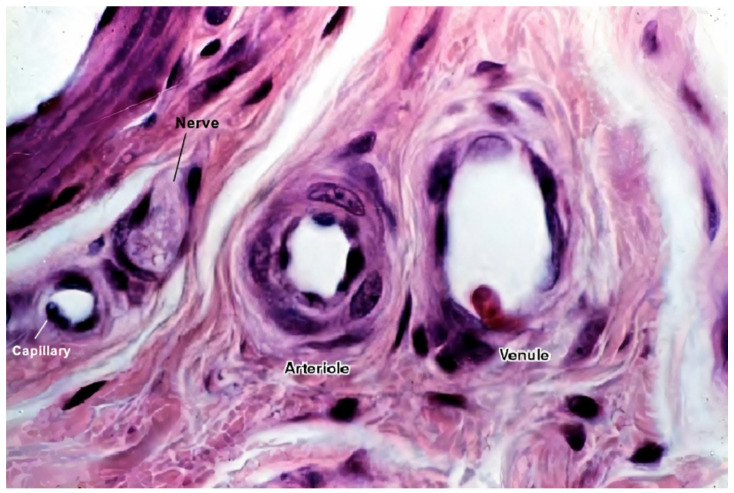
\includegraphics[scale=0.7]{gambar/mikrovaskular.jpg}
	\caption{ Sistem Mikrovaskular \cite{guven_microcirculation_2020}}
	\label{fig:mikrovaskular}
\end{figure}


\noindent Mikrovaskular merupakan cabang terkecil dari pembuluh darah, memainkan peran penting dalam sirkulasi darah dan pertukaran zat di seluruh tubuh \cite{rusanova_role_2022}. Struktur ini, dengan ukuran kurang dari 100 mikrometer, terdiri dari arteriol, kapiler dan venula \cite{mescher_junqueiras_2021,pepe_microvascular_2023}. Arteriol merupakan pembuluh darah berdiameter 10-100 $\mu$m yang bertindak sebagai pengatur tekanan darah. Kapiler merupakan pembuluh darah berdiameter 4-10 $\mu$m yang berfungsi sebagai tempat pertukaran metabolit antara darah dan jaringan \cite{haffner_emerging_2023}. Venula merupakan pembuluh darah berdiameter 10-100 $\mu$m tempat berlanjutnya aliran darah dari kapiler dan membawanya ke vena. Struktur ini juga berperan sebagai tempat keluarnya leukosit (sel darah putih) untuk mengatasi infeksi atau peradangan pada jaringan.


\noindent Studi tentang mikrovaskular sangat penting dalam bidang kesehatan dan patologi. penelitian internasional yang sedang berlangsung \textit{Human Cell Atlas }(HCA) oleh Chan Zuckerberg Initiative, \textit{Human Protein Atlas} (HPA) oleh Knut and Allice Wallenberg Foundation dan \textit{Human BioMolecular Atlas Program} (HuBMAP) oleh National Institutes of Health menggunakan kerangka kerja yang bernama \textit{Vascular Common Coordinate Framework} (VCCF) yang memanfaatkan pembuluh darah sebagai sistem koordinat dalam tubuh manusia untuk memetakan setiap sel di seluruh tubuh manusia \cite{weber_considerations_2020,zhao_attention-based_2023}. penelitian tersebut dilakukan untuk memahami spesialisasi, interaksi dan organisasi spasial setiap sel dalam tubuh manusia.

\noindent Pemanfaatan mikrovaskular sebagai kordinat pada kerangka kerja VCCF tersebut bisa dilakukan karena pembuluh darah  mengikuti setiap jalur unik di setiap organ sehingga bisa mencerminkan sifat biologis khusus setiap jaringan \cite{weber_considerations_2020}. Kerumitan struktur mikrovaskular mencerminkan kompleksitas organ dan jaringan yang dilaluinya, sehingga dapat menyoroti ketergantungan antara mikrovaskular dan sel dalam menjalankan fungsi yang tepat. 



\section{Ginjal dan Mikrovaskular Ginjal}


Ginjal adalah organ vital yang bertanggung jawab untuk menyaring darah, mengatur tekanan darah, dan menjaga keseimbangan elektrolit dalam tubuh manusia \cite{sultan_microvasculature_2023,ito_s-27-1_2023,bagarao_renal_2023}. %+\citeabdulla_biology_2022
Ginjal melakukan hal tersebut melalui proses-proses seperti filtrasi glomelurus, penyerapan tubulus, dan sekresi tubulus, yang pada akhirnya membentuk urin \cite{auctores_publishing_llc_what_2021}. Kemudian, ginjal membantu mengatur volume cairan tubuh, kandungan elekrolit, dan keasaman, serta membuang produk limbah dan racun dalam tubuh. Secara garis besar, ginjal sangat penting untuk menjaga lingkungan internal tubuh, guna menjamin kondisi yang optimal agar berbagai proses tubuh dapat berfungsi dengan baik.
 

\noindent Fungsi-fungsi vital ginjal dilakukan oleh struktur-struktur khusus di dalamnya, terutama pada bagian korteks, medula, dan papila. Masing-masing bagian ini memiliki peran unik dalam proses filtrasi, reabsorpsi dan sekresi yang terjadi di ginjal. korteks merupakan area terluar ginjal yang memiliki sel-sel bulat ginjal yang membungkus glomelurus sebagai alat untuk menyaring darah \cite{gopalan_renal_2022,mescher_junqueiras_2021}. Medula merupakan area dalam dalam ginjal terdiri dari tubulus-tubulus nefron (lengkung Henle dan duktus kolektivus) dan pembuluh struktur kapiler khusus medula bernama vasa recta yang berperan dalam pengatur konsentrasi urin \cite{haug_multi-omic_2022}. Papila merupakan sub bagian dari medula yang merupakan dasar dari piramida ginjal berfungsi sebagai tempat pengumpulan urin sebelum di teruskan ke kaliks minor \cite{sabate_arroyo_relationship_2020}.

\noindent Mikrovaskular ginjal memiliki beberapa komponen unik yang berperan penting dalam proses pembentukan urin dan pengaturan fungsi ginjal, mencakup glomelurus, kapiler peritubular, vasa recta, arteriol aferen dan arteriol eferen \cite{mescher_junqueiras_2021}. Glomelurus merupakan kumpulan kapiler yang terdapat di kapsul Bowman yang berfungsi sebagai alat penyaring darah sehingga air dan limbah bisa melewati dinding kapiler ke dalam kapsul Bowman, sementara sel darah dan protein besar tetap berada di dalam aliran darah \cite{luxen_unique_2023}. kapiler peritubular merupakan kapiler yang mengelilingi tubulus ginjal yang berperan mereabsorsi cairan penting yang tidak tersaring di dalam glomelurus \cite{savedchuk_targeting_2023}. Vasa recta merupakan kapiler yang terletak di medula ginjal, mengelilingi  lengkung henle yang berfungsi menjaga gradien osmotik untuk proses reabsorsi air dari duktus kolektivus \cite{goligorsky_emerging_2022}. Arteriol aferen dan eferen merupakan arteriol  yang berfungsi dalam transportasi darah dari dan ke glomlurus \cite{ergin_kidney_2021}.



\section{Whole Slides Image (WSI)}

\noindent \textit{Whole Slide Image} (WSI) merupakan teknologi dalam pengambilan gambar histologi yang melibatkan pemindaian slide mikroskopik menjadi gambar digital beresolusi tinggi \cite{hanna_whole_2020}. Gambar yang dihasilkan dari pemindaian WSI biasanya berukuran besar (ratusan hingga ribuan megabyte) yang di simpan dalam berbagai format, termasuk \textit{Scope Virtual Slide} (SVS), \textit{MIRAX Slide Image} (MRXS), \textit{NanoZoomer Digital Pathology Image} (NDPI), \textit{Tagged Image File Format} (TIFF), dan \textit{Digital Imaging and Communications in Medicine }(DICOM). Penggunaan WSI dalam pemindaian slide mikroskopik ini dapat meningkatkan reproduksibilitas analisis dan mengurangi kesalahan manusia dalam interpretasi visual \cite{li_hardware-software_2023}. Dalam dunia patologi WSI juga dimanfaatkan untuk berbagai keperluan termasuk: diagnosis primer dimana dalam pembuatan diagnosis tanpa melihat ke dalam slide kaca secara langsung, konsultasi jarak jauh dengan berbagai WSI secara digital dan penelitian yang melibatkan analisis WSI untuk penelitian biomolekular, penemuan obat baru dan pengembangan alat diagnostik.

\begin{figure}[h]
	\centering
	\begin{subfigure}[b]{0.3\textwidth}
		\centering
		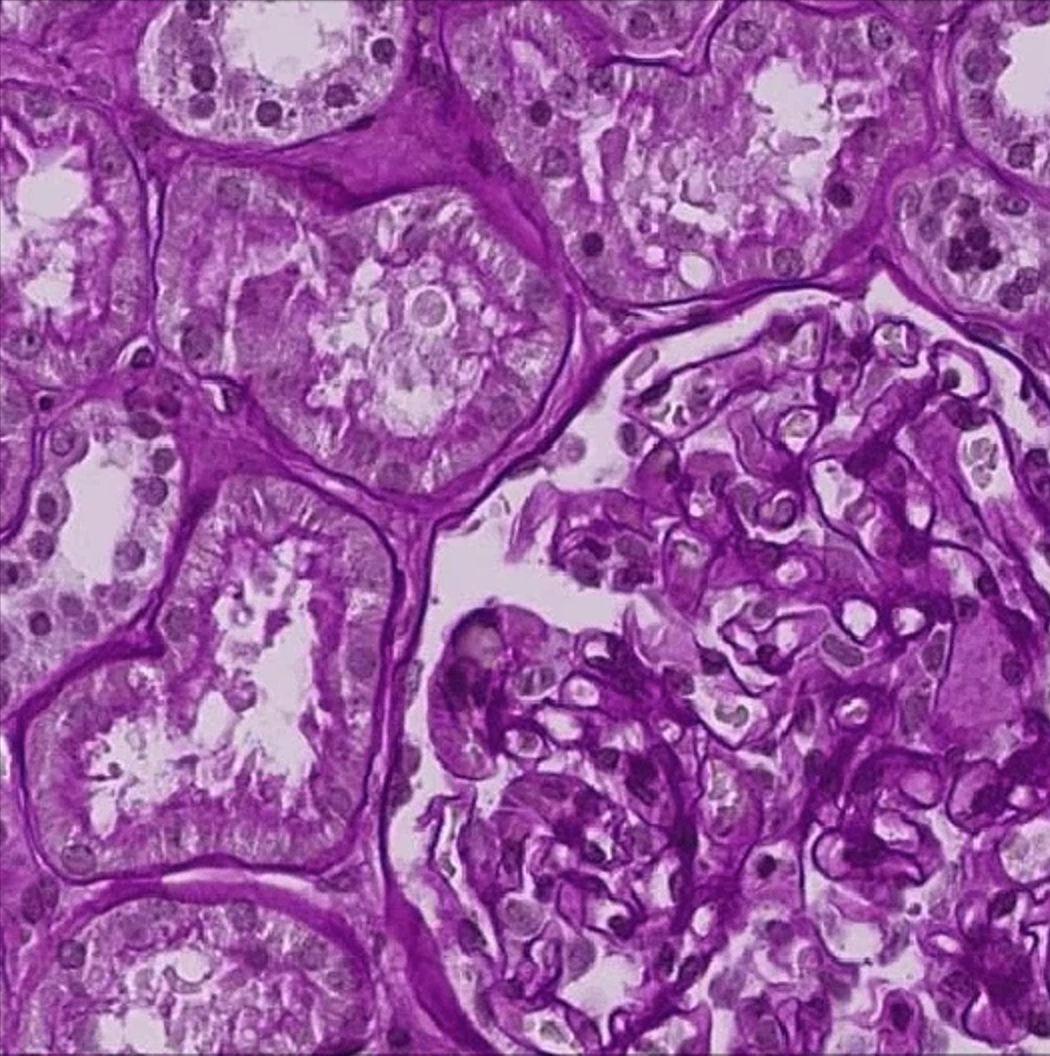
\includegraphics[width=\textwidth]{gambar/korteks.png}
		\caption{Korteks}
		\label{fig:korteks}
	\end{subfigure}
	\hfill
	\begin{subfigure}[b]{0.3\textwidth}
		\centering
		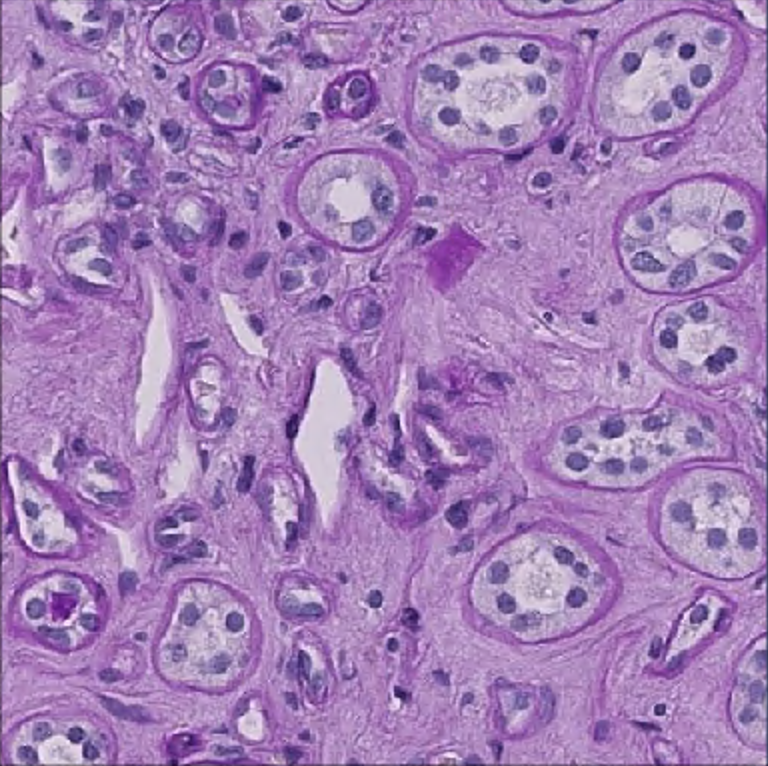
\includegraphics[width=\textwidth]{gambar/medula.png}
		\caption{Medula}
		\label{fig:medula}
	\end{subfigure}
	\hfill
	\begin{subfigure}[b]{0.3\textwidth}
		\centering
		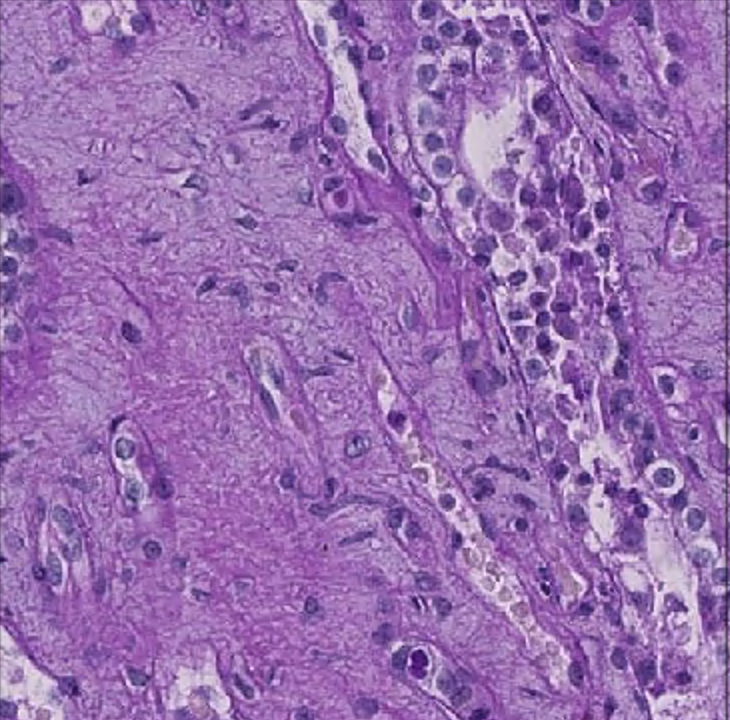
\includegraphics[width=\textwidth]{gambar/papila.png}
		\caption{Papila}
		\label{fig:papila}
	\end{subfigure}
	\caption{Sample WSI pada bagian ginjal \cite{howard_hubmap_2023}}
	\label{fig:ginjal}
\end{figure}

 
\section{Segmentasi Gambar}

\noindent Segementasi gambar merupakan sebuah tugas penting dalam anilisis gambar histologis dan medis. Proses ini akan mempartisi gambar digital menjadi wilayah yang terpisah (tidak tumpang tindih), yang masing-masing wilayah  berhubungan dengan suatu objek atau struktur yang relevan dalam lingkup pengamatan \cite{wu_image_2023}. Dengan kata lain, segmentasi gambar merupakan proses mengelompokkan piksel-piksel dalam gambar berdasarkan karakteristik tertentu. Hasil dari segmentasi gambar adalah sekumpulan segmen yang mewakili objek dari objek yang berbeda dalam gambar. Metode yang di gunakan dalam proses ini sangat bervariasi, dari yang metode sederhana seperti: \textit{treshholding} memisahkan piksel berdasarkan intensitasnya, \textit{region growing} mengelompokkan piksel-piksel berdasarkan kemiripan, \textit{clustering} memisahkan piksel berdasarkan kemiripan dalam fitur multidimensi dan \textit{aktive countour} menggunakan kurva yang dapat berubah untuk mendeteksi objek, hingga metode \textit{deep learning} seperti model FCN yang lebih canggih \cite{huang_fully_2022,wang_comprehensive_2022}.

\noindent Dalam praktiknya segmentasi gambar menggunakan \textit{deep learning} terbagi ke dalam dua jenis: segmentasi semantik dan segmentasi instance. Segmentasi semantik merupakan jenis segmentasi untuk mencari pemahan rinci terhadap berbagai wilayah dalam gambar yang mana pada jenis ini pelabelan setiap piksel dalam gambar didasarkan setiap kelas objek \cite{fan_image_2023}. Di sisi lain, segmentasi instace melabeli piksel objek dalam gambar tidak hanya didasarkan setiap kelas dari objek tetapi, juga membedakan antara instance objek  secara individu walaupun ada dalam kelas yang sama sehingga memungkinkan untuk penggambaran yang tepat dari setiap objek yang ada dalam gambar. Kedua jenis segmentasi ini telah dimanfaatkan dalam berbagai bidang seperti analisis citra lalulintas untuk sistem kemudi otomatis, transfer gaya gambar dalam komputer vision dan analisis struktur mikrovaskular sebagaimana yang akan dilakukan pada penelitian ini \cite{wang_traffic_2023, zhang_image_2023, sultan_microvasculature_2023}


\section{Deep Learning}

\noindent Deep learning merupakan sub bidang dari machine learning yang menggunakan jaringan syaraf tiruan dengan banyak layer untuk mempelajari pola dari suatu data \cite{goodfellow_deep_2016,yang_deep_2023}. Perkembangan deep learning memberikan pengaruh besar pada analisis citra medis \cite{sistaninejhad_review_2023}. Dimana pada tahap awal perkembangan analisa citra medis, fitur-fitur diektraksi secara tradisional menggunakan teknik pemrosesan citra tradisional yang memakan waktu dan butuh validasi ahli \cite{huang_fully_2022}.  Kemudian, dengan munculnya deep leaning terutama \textit{Convolutional Neural Network} (CNN), proses ektraksi fiturpun menjadi otomatis \cite{huang_fully_2022,azad_medical_2022}. 

\begin{figure}[H]
	\centering
	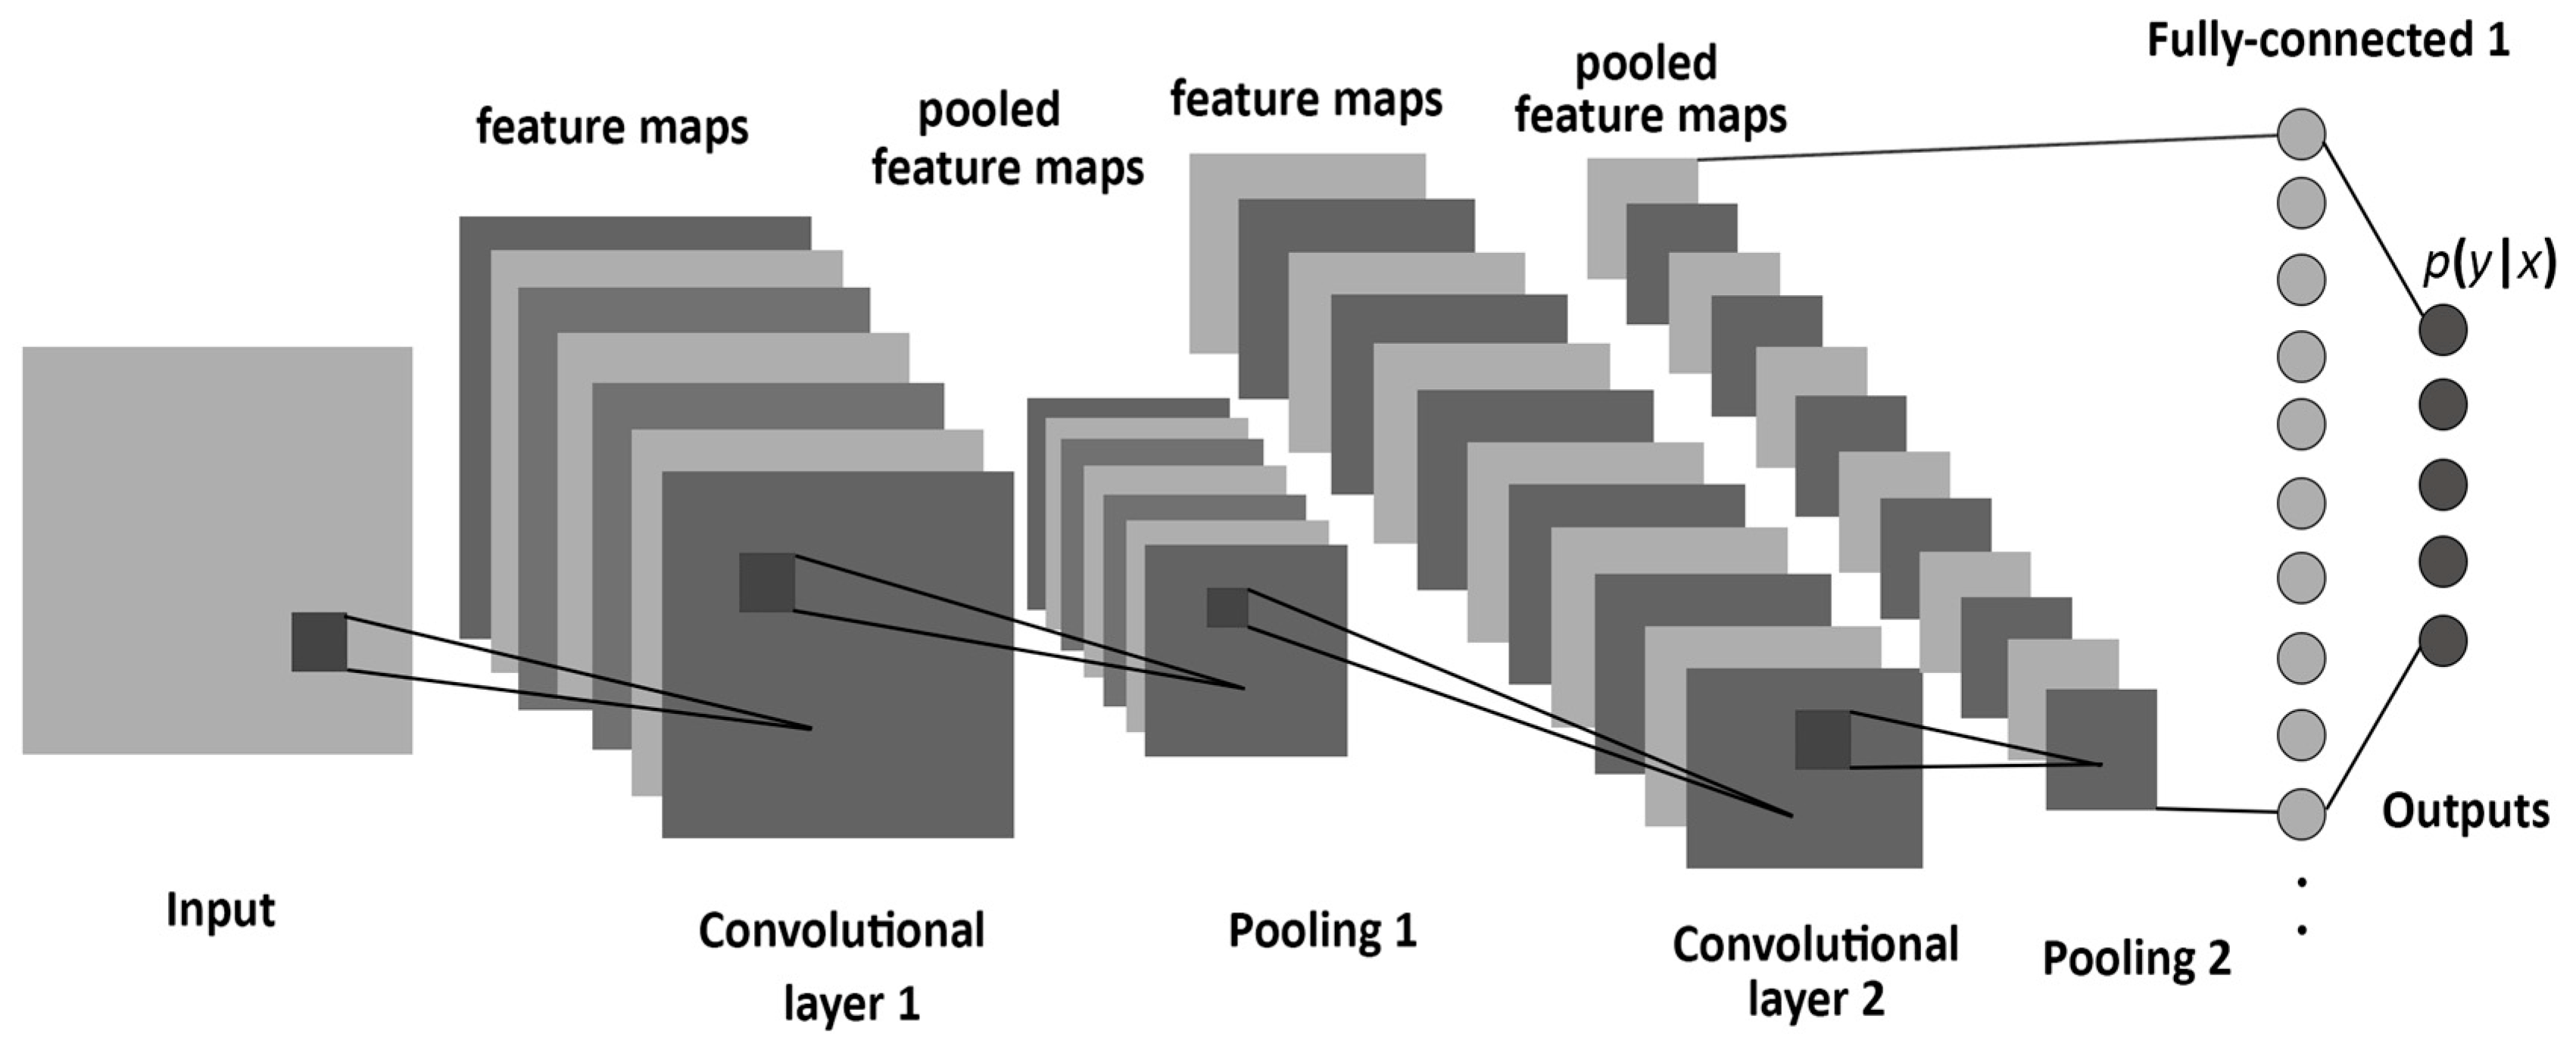
\includegraphics[scale=.08]{gambar/CNN.PNG}
	\caption{Model CNN \cite{albelwi_framework_2017}}
	\label{fig:CNN}
\end{figure}

\noindent CNN merupakan model jaringan saraf tiruan yang sangat efektif untuk tugas-tugas pengolahan citra, seperti klasifikasi gambar dan objek deteksi pada gambar \cite{celeghin_convolutional_2023}. CNN bekerja dengan cara mengekstraksi fitur-fitur penting dari gambar melalui serangkaian lapisan konvolusi, \textit{pooling}, dan fungsi aktivasi, yang memungkinkan model untuk mengenali pola dan struktur dalam data visual. Namun CNN tradisional memiliki keterbatasan untuk tugas segmentasi  gambar \cite{huang_fully_2022, azad_medical_2022, jasim_towards_2023}. Salah satunya berkaitan dengan fitur yang di ekstraksi model tersebut. Ketika menggunakan kernel yang lebih kecil, fitur yang di hasilkan akan lebih lokal terhadap gambar asli, sehingga informasi global seperti lokasi mungkin hilang. Namun, ketika menggunakan kernel yang lebih besar, konteks dari fitur lokal tersebut dapat berkurang. Untuk mengatasi masalah tersebut Long et al. (2014) \cite{long_fully_2014} memperkenalkan model \textit{Fully Convolutional Network} (FCN) yang lebih cocok untuk tugas segmentasi, karena terdiri dari struktur \textit{encoder-decoder} untuk secara bertahap mengurangi resolusi gambar (downsampling) dan kemudian meningkatkannya kembali (upsampling), memungkinkan model untuk menangkap fitur pada berbagai skala dan mempertahankan informasi spasial.


\subsection{Fully Convolutional Network (FCN)}

Salah satu model \textit{deep learning} yang sering digunakan dalam tugas segmentasi merupakan \textit{Fully Convolutional Network }(FCN). Perbedaan utama antara \textit{Convolutional Neural Network} (CNN) tradisional dan FCN terletak pada lapisan terakhir. CNN tradisional menggunakan \textit{fully connected layer} atau jaringan dense untuk mengintegrasikan informasi sebelum menghasilkan output. Sebaliknya, FCN mengganti lapisan terakhir tersebut dengan jaringan konvolusi untuk menghasilkan output channel \cite{shlezinger_model-based_2023,huang_fully_2022}. Salah satu manfaat utama dari pendekatan ini adalah bahwa model tidak akan mendapatkan pembatasan dari \textit{fully connected layer}, sehingga ukuran dari output	 akan lebih fleksibel \cite{iqbal_analyses_2023}.


Struktur FCN seperti pada gambar \ref{fig:fcn} menerapkan beberapa blok konvolusi yang terdiri dari lapisan konvolusi, aktivasi dan \textit{pooling} pada jalur encoder untuk menangkap representasi semantik dari gambar \cite{azad_medical_2022}. Begitu juga, dalam jalur decoding FCN menggunakan lapisan konvolusi bersamaan dengan operasi \textit{upsampling} untuk memberikan prediksi pada tingkat piksel sehingga model bisa melakukan tugas segmentasi \cite{deng_fcn_2023}. \textit{Skip conections} juga digunakan dalam FCN untuk menemukan lokasi dari fitur di keseluruhan citra. 

\begin{figure}[H]
	\centering
	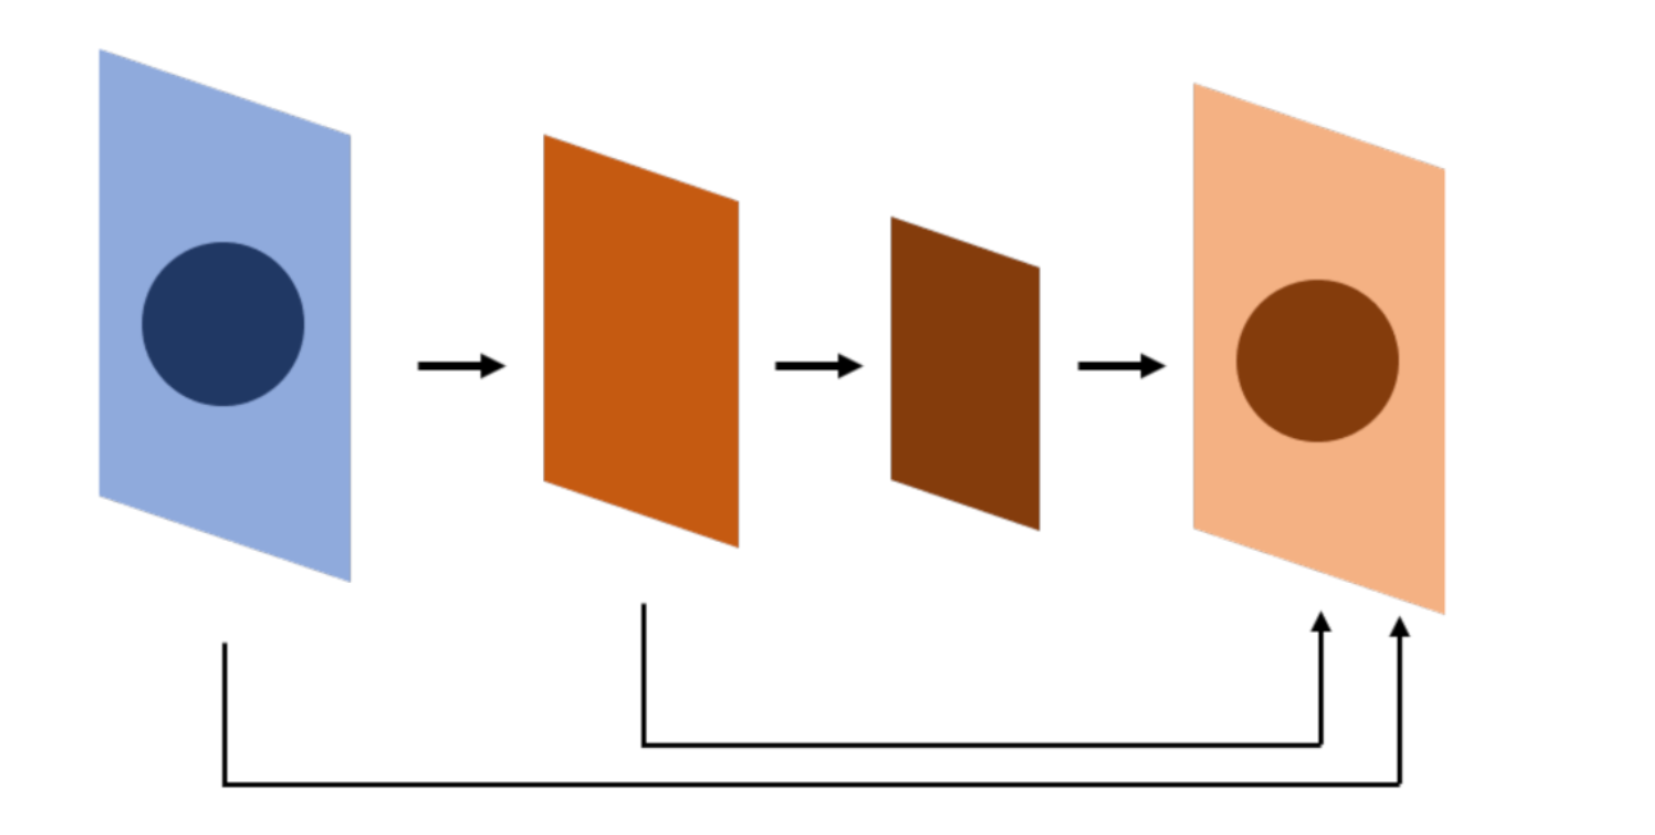
\includegraphics[scale=.2]{gambar/gambar-fcn.png}
	\caption{Model FCN yang bagian terakhirnya di gantikan dengan blok konvolusi \cite{huang_fully_2022}}
	\label{fig:fcn}
\end{figure}


\subsection{U-Net}

\noindent Arstitektur FCN yang terdiri dari bagian \textit{encoder-decoder}, khusus digunakan dalam tugas segmentasi citra biomedis adalah U-Net yang pertama kali dikenalkan oleh Ronneberger et al.(2015) \cite{ronneberger_u-net_2015}. Arsitektur ini menjadi cukup populer di kalangan peneliti, terutama bidang analisis citra biomedis, karena kemampuannya untuk memberikan hasil segmentasi yang akurat dengan jumlah data pelatihan yang relatif kecil \cite{williams_unified_2023}.

\begin{figure}[H]
	\centering
	\includegraphics[scale=.2]{gambar/U-Net.png}
	\caption{Arsitektur dasar U-Net yang digunakan untuk tugas segmentasi citra biomedis \cite{ronneberger_u-net_2015}}
	\label{fig:U-net}
\end{figure}

\noindent U-Net memanfaatkan ekstraksi fitur dari jaringan konvolutional, dimana lapisan \textit{upsampling} dan \textit{skip connection} digunakan untuk membandingkan fitur dari lapisan atas sambil tetap mempertahankan fitur dari lapisan bawah \cite{huang_fully_2022}. Dengan demikian, model mampu mendeteksi fitur-fitur detail dan umum dari objek, sehingga bisa mendeteksi objek secara akurat. U-Net dapat disebut sebagai metode klasifikasi tingkat piksel, dimana segmentasi dilakukan melalui klasifikasi piksel per piksel \cite{siddique_u-net_2020}. Struktur arsitektur dari U-Net akan dijelaskan secara singkat sebagai berikut:

\begin{itemize}
	\item Bagian pertama dari arsitektur U-Net adalah bagian menurun yang dikenal juga sebagai bagian \textit{encoder} yang berfungsi untuk menangkap informasi kontekstual gambar \cite{azad_medical_2022}. Bagian ini terdiri dari unit-unit blok konvolusi, dimana setiap blok berisi dua \textit{convolution layers} 3x3 berurutan dan \textit{pooling layers} yang mirip dengan CNN konvensional, kadang juga menyertakan juga menyertakan \textit{batch normalization layers} \cite{younisse_fine-tuning_2023}. Sebelum memasuki \textit{pooling layers}, fitur akan difilter terlebih dahulu melalui fungsi aktivasi ReLu untuk menentukan apakah fitur yang diekstraksi akan ditransfer ke layer selanjutnya.
	
	\item Bagian kedua adalah bagian mendaki yang dikenal juga sebagai bagian \textit{decoder} yang bertujuan untuk secara bertahap meningkatan pemetaan fitur ke resolusi yang diinginkan\cite{siddique_u-net_2020}. Bagian ini terdiri dari layer \textit{transpose convolution} 2x2 (atau deconvolution) yang berfunsi sebagai \textit{upsampling} untuk mengembalikan dimensi spasial yang hilang selama proses pooling pada bagian encoder. Kemudian, diikuti dua \textit{convolution layers} 3x3 berurutan untuk memperbaiki fitur yang telah di-\textit{upsampling} untuk memastikan detail spasial tetap terjaga dan diperbaiki\cite{purushothaman_image_2022}. Fungsi aktivasi ReLu juga digunakan pada bagian ini setelah setiap operasi konvolusi untuk memperkenalkan non-linieritas yang memungkinkan jaringan untuk mempelajari representasi yang lebih kompleks dan akurat pada resolusi yang lebih tinggi\cite{huang_fully_2022}.
	
	\item Diantara \textit{encoder} dan \textit{decoder} terdapat \textit{bottleneck} yang terdiri dari \textit{convolution layers} 3x3 berurutan dengan fungsi aktivasi ReLu \cite{azad_medical_2022}. Bagian ini berfungsi untuk menangkap fitur pada resolusi terendah dan menghubungkan informasi dari \textit{encoder} dan \textit{deceoder}.
	
	\item \textit{Skip connection} dari \textit{encoder} ke \textit{decoder} digunakan juga pada U-Net untuk meningkatkan kinerja model pada tugas segmentasi gambar \cite{azad_medical_2022}. \textit{Skip connection}  merupakan jalur langsung yang menghubungkan layer pada bagian \textit{encoder} dengan layer pada bagian \textit{decoder} pada tingkat resolusi yang sama. Dengan penggunaan \textit{skip connection} memungkinkan model untuk mempertahankan fitur resolusi tinggi dari gambar input yang mungkin hilang selama proses \textit{downsampling} di \textit{encoder}. Kemudian,\textit{ skip connection} juga mepertahankan informasi lokasi yang membantu dalam rekontruksi fitur yang lebih akurat\cite{siddique_u-net_2020}.
	
	\item \textit{Output layers}  pada arsitektur U-Net ini merupakan sebuah \textit{convolutional layer} 1x1 yang berada di puncak decoder berfungsi untuk menghasilkan prediksi piksel per piksel \cite{huang_fully_2022,azad_medical_2022}. Fungsi aktivasi Softmax sering diterapkan pada layer output untuk menghasilkan distribusi probabilitas setiap kelas pada setiap piksel. Namun, untuk data yang terdiri dari dua kelas lebih umum digunakan fungsi aktivasi sigmoid.
	
	
\end{itemize}



\section{Modul Attention Gate (AG)}

\noindent Penggunaan modul \textit{Attention Gate} (AG) pertamakali digunakan dalam \textit{deep learning} di pemrosesan bahasa alami (natural language proccessing)\cite{azad_medical_2022}. Modul ini mencari korelasi antara query dan key untuk mendapatkan bobot yang sesuai dengan kata kunci. Hasilnya, AG ini dapat menangkap hubungan antara teks dalam suatu wilayah atau paragraf dengan lebih tepat. Konsep serupa juga bisa digunakan dalam \textit{computer vision} \cite{huang_fully_2022}. Menerapkan AG dapat membuat model menggabungkan korelasi fitur-fitur regional, sehingga menghasilkan hasil deteksi tepi objek yang lebih baik untuk meningkatkan kinerja.



\noindent Citra biomedis memiliki variasi tinggi dalam bentuk dan ukuran. Pendekatan umum yang biasanya dilakukan untuk menghadapi masalah ini adalah susunan \textit{cassaded network}, dimana jaringan pertama  mengekstraksi \textit{region of interest} (ROI) termasuk organ yang akan di segmentasi, dan jaringan kedua meprediksi segmentasi organ yang tepat di dalam ROI \cite{oktay_attention_2018}. Namun, pendekatan ini sering mengalami redudansi parameter model dan kebutuhan sumber daya komputasi yang tinggi. Dengan menambahkan AG pada U-Net seperti pada gambar \ref{fig:Attention-U-net}, model dapat secara efektif menekankan fitur-fitur yang relevan tanpa memerlukan jaringan terpisah untuk prediksi ROI, sehingga mengurangi redundansi parameter dan meningkatkan efisiensi komputasi\cite{azad_medical_2022}.

\begin{figure}[H]
	\centering
	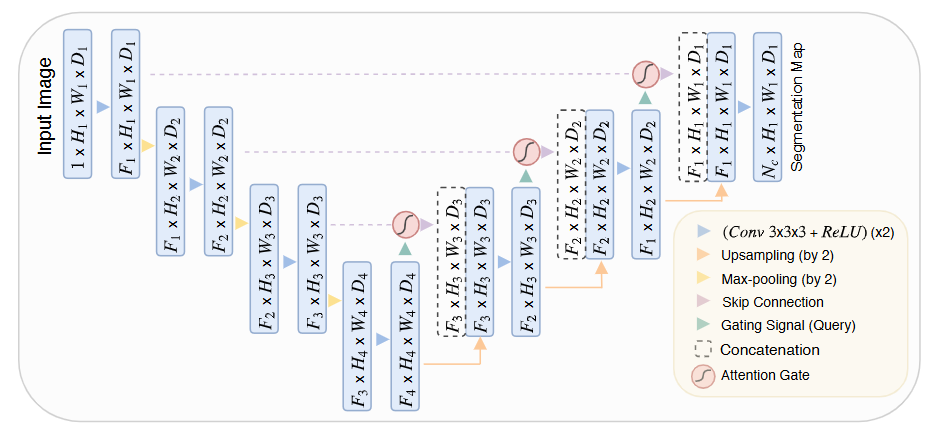
\includegraphics[scale=.5]{gambar/AG-U.png}
	\caption{Diagram Attention U-Net untuk tugas segmentasi \cite{oktay_attention_2018}}
	\label{fig:Attention-U-net}
\end{figure}



Diagram pada gambar \ref{fig:AG} menunjukkan skema kerja AG dalam Attention U-net.AG berfungsi untuk untuk menyoroti fitur-fitur penting yang melewati \textit{skip connections} \cite{siddique_u-net_2020,oktay_attention_2018}. Pertama, fitur input dari layer \(l\) (\(x^l\))  dan sinyal \textit{gating} (\(g\)) yang dikumpulkan dari skala kasar dipetakan ke ruang dimensi yang lebih rendah menggunakan transformasi linier menggunakan konvolusi 1x1x1 secara terpisah. Kemudian, fitur-fitur tersebut ditambahkan dan dilewatkan melalui fungsi aktivasi \textit{Rectified Linear Unit} (ReLU($\sigma1$)) untuk menghasilkan fitur yang lebih terfokus. Setalah itu, hasilnya dilewatkan melalui transformsi linier lain ($\psi$) dengan konvolusi 1x1x1 dan fungsi aktivasi sigmoid ($\sigma1$) untuk mendapatkan koefisien perhatian ($\alpha$). Koefisien perhatian ini kemudian di-resample ke ukuran grid yang sama dengan fitur input asli menggunakan interpolasi bilinier. Fitur input asli \(x^l\) kemudian diskalakan dengan koefisien perhatian yang telah di-resample, menghasilkan output akhir $\hat{x}^l$. Proses ini memastikan bahwa hanya fitur-fitur yang relevan yang diteruskan, sementara yang tidak relevan diabaikan.

\begin{figure}[H]
	\centering
	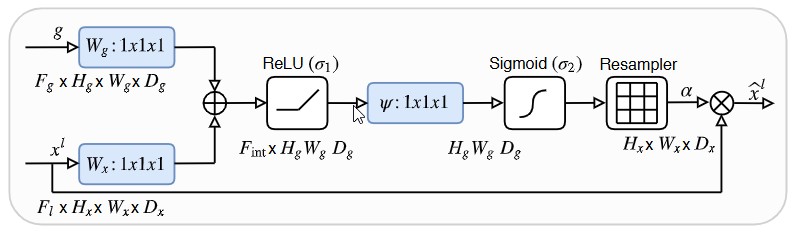
\includegraphics[scale=.5]{gambar/AG.png}
	\caption{Diagram alur kerja Attention Gate \cite{oktay_attention_2018}}
	\label{fig:AG}
\end{figure}

\section{Konvolusi, Pooling dan Transpose Konvolusi}

\noindent Konvolusi, pooling dan transpose konvolusi merupakan lapisan operasi yang digunakan bersama-sama dalam \textit{deep learning}, termasuk U-Net \cite{goodfellow_deep_2016,pajankar_convolutional_2022,bishop_deep_2024}.  Lapisan konvolusi bertindak sebagai pengekstraksi fitur, lapisan pooling berfungsi untuk mengurangi dimensi peta fitur, sedangkan dekonvolusi berfungsi untuk meningkatkan dimensi di bagian \textit{encode}r. 

\subsection{Konvolusi}

\begin{figure}[H]
	\centering
	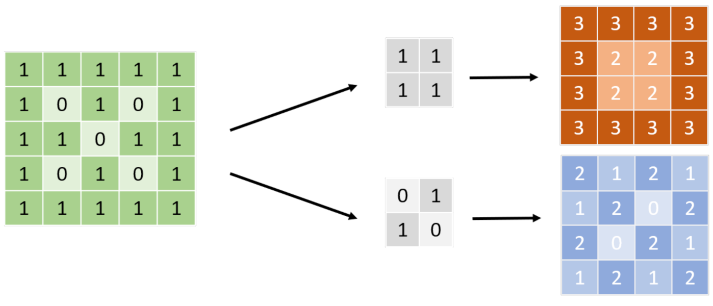
\includegraphics[scale=.3]{gambar/convolusi.png}
	\caption{Penerapan konvolusi terhadap input \cite{huang_fully_2022}}
	\label{fig:convolusi}
\end{figure}

\noindent Konvolusi adalah operasi matematika dimana sebuah kernel (atau filter) digeserkan pada bagian gambar input untuk memproduksi \textit{feature map} (peta fitur) \cite{pajankar_convolutional_2022}.  Pada gambar menunjukkan kernel yang berbeda akan menghasilkan peta fitur yang berbeda juga. Dalam library \textit{deep learning} operasi  konvolusi yang digunakan disebut \textit{cross-corrlelation}\cite{goodfellow_deep_2016}. Dengan formula sebagai berikut:

\begin{equation}
	C(i, j) = (I * K)(i, j) = \sum_{m} \sum_{n} I(i - m, j - n) K(m, n)
\end{equation}


\noindent
keterangan:
\begin{itemize}
	\item $C(i,j)$ : hasil konvolusi pada posisi $(i,j)$
	\item $I(i-m, j-n)$ : nilai piksel citra masukan pada posisi $(i-m, j-n)$
	\item $K(m,n)$ : nilai pada filter di posisi $(m,n)$
\end{itemize}

\subsection{Pooling}

\noindent Fungsi pooling merupakan sebuah fungsi untuk mengubah \textit{output} jaringan di lokasi tertentu menjadi ringkasan statistik dari \textit{output} terdekat\cite{goodfellow_deep_2016,bishop_deep_2024}. Fungsi ini berguna untuk melakukan down-sampling pada peta fitur, yang berarti mengurangi dimensi peta fitur sambil tetap mempertahankan informasi penting. \textit{Down-sampling} ini mengenalkan \textit{invariance} pada jaringan \cite{goodfellow_deep_2016}. Sehingga jaringan bisa melihat fitur mana yang lebih sering muncul, tanpa tergantung pada lokasi aslinya.

\noindent Jenis pooling yang sering digunakan dalam deep learning meliputi \textit{max pooling}, yang mengambil nilai maksimum dari area yang dipilih \cite{bishop_deep_2024}. Kemudian ada \textit{average pooling} yang mengambil rata-rata dari nilai-nilai di area tersebut \cite{bishop_deep_2024}. Dalam arsitektur U-net, \textit{max pooling} digunakan karena efektif dalam mempertahankan fitur-fitur dominan yang penting untuk segmentasi.

\begin{figure}[H]
	\centering
	\includegraphics[scale=0.5]{gambar/figure_8.pdf}
	\caption{Pnerapan pooling terhadap peta fitur \cite{bishop_deep_2024}}
	\label{fig:pooling}
\end{figure}

\subsection{Transpose Konvolusi}


\noindent Transpose konvolusi atau dekonvolusi merupakan fungsi yang digunakan untuk meningkatkan dimensi peta fitur \cite{goodfellow_deep_2016,bishop_deep_2024}. Pada arsitektur U-Net fungsi ini digunakan pada bagian \textit{up-sampling} untuk mengembalikan ukuran peta fitur yang telah melalui bagian \textit{down-sampling} \cite{azad_medical_2022}. Cara kerja operasi ini adalah dengan menerapkan filter yang terhubung dengan satu piksel di tensor input pada patch yang ada di tensor output. Secara matematis proses dekonvolusi dapat dirumuskan sebagai berikut:

\begin{equation}
	I(i,j) = (C * K^T)(i,j) = \sum_{m} \sum_{n} C(m, n) K(i - m, j - n)
\end{equation}

\noindent
keterangan:
\begin{itemize}
	\item $I(i,j)$ : nilai pada posisi $(i,j)$ dari hasil transpose convolution
	\item $C(m,n)$ : nilai pada posisi $(m,n)$ dari input
	\item $K(i-m, j-n)$ : nilai pada posisi $(i-m, j-n)$ dari kernel/filter yang diterapkan terbalik
\end{itemize}


\begin{figure}[H]
	\centering
	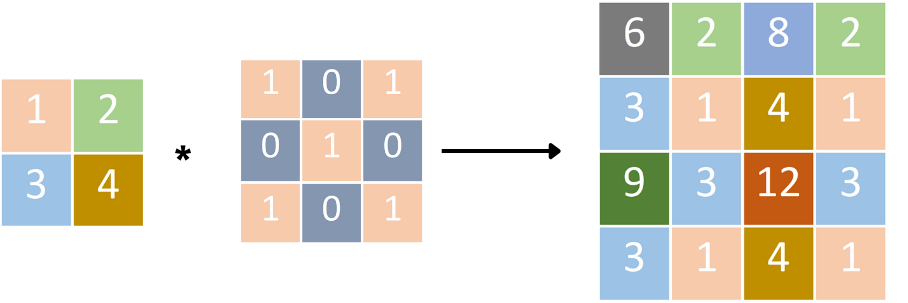
\includegraphics[scale=0.5]{gambar/deconv.png}
	\caption{Transpose konvolusi dari peta fitur \cite{bishop_deep_2024}}
	\label{fig:deconv}
\end{figure}


\section{Augmentasi Data}

\noindent Teknik augmentasi data merupakan salah satu metode yang umum digunakan untuk meningkatkan peforma model deep learning \cite{minaee_image_2020}. Augmentasi data memungkinkan model untuk menghasilkan data baru yang tetap menyerupai data orisinal, tetapi dipandang berbeda oleh model selama pelatihan \cite{huang_fully_2022}. Data augmentasi bisa meningkatkan variasi dari data dan mengurangi gap antara data latih dan uji untuk meningkatkan ketahanan model.

\noindent Dalam pencitraan biomedis augmentasi sering digunakan dalam tugas segmentasi karena ketidakseimbangan antar kelas dalam tugas segmentasi. Oleh karena itu, lebih baik mempertahankan gambar asli fitur untuk konvergensi model. Dalam penerapannya augmentasi biasanya berupa transformasi gemoetris acak (rotation, scaling, shear dan flipping) dan modifikasi intensitas acak (normalization, blurring dan penyesuaian contrast)\cite{minaee_image_2020}.

\section{Oversampling}

\noindent Oversampling merupakan salah satu teknik yang umum dilakukan peneliti dalam menghadapi masalah ketidakseimbangan kelas dalam dataset. Teknik ini bertujuan untuk meningkatkan jumlah sampel dari kelas minoritas dengan mereplikasi sampel-sampel dari kelas tersebut secara acak \cite{bria_addressing_2020}. Dalam konteks segmentasi gambar, oversampling memungkinkan model untuk "melihat" lebih banyak contoh dari objek yang jarang atau kurang terwakili, sehingga model dapat lebih mudah mengenali fitur-fitur dari kelas minoritas. Teknik ini sering dikombinasikan dengan data augmentation yang menambah variasi pada gambar yang dioversample, seperti flipping, rotasi, dan zooming, agar model dapat belajar dengan lebih robust dan menghindari resiko overvitting dari data yang sama.


\section{Fungsi Aktivasi}

\noindent Fungsi aktivasi digunakan dalam \textit{deep learning} untuk memperkenalkan non-linieritas kepada sebuah jaringan, memungkinkan jaringan mengenali kompleksitas dari sebuah data \cite{younisse_fine-tuning_2023,heaton_ian_2018}. Tanpa adanya fungsi aktivasi, jaringan hanya akan menjadi representasi linier dari seluruh data yang dilatih \cite{chiang_activation_2023}. Selain itu, juga akan menyebabkan masalah seperti \textit{vanishing gradient} (gradien yang hilang) atau \textit{exploding gradient} (gradien yang meledak), yang akan menghambat proses pembelajaran jaringan. Salah dua fungsi aktivasi yang sering digunakan dalam arsitektur jaringan U-net adalah \textit{Rectified Linear Unit} (ReLU) dan \textit{sigmoid}. %Penjelasan singkat dari keduanya adalah sebagai berikut ini:

\subsection{ReLU:}
Merupakan singkatan dari \textit{rectified linear unit}. Cara kerja dari fungsi aktivasi ini cukup sederhana, jika input (x) adalah positif maka outputnya adalah nilai itu sendiri \cite{younisse_fine-tuning_2023}. Jika inpuntya negatif atau nol maka outputnya adalah nol. Dengan kata lain, fungsi aktivasi ReLU mengaktifkan neuron dengan input positif dan menonaktifkan selainnya. secara matematis fungsi ReLU adalah sebagai berikut ini: 

\begin{equation}
	\sigma(x) = \max(0, x)
\end{equation}

\noindent
keterangan:
\begin{itemize}
	\item $x$ : nilai piksel setiap \textit{feature map} yang dihasilkan lapisan konvolusi
	\item $\max$ : fungsi yang akan memilih nilai terbesar antara 0 dan nilai $x$
\end{itemize}

\subsection{Sigmoid:}
Merupakan fungsi aktivasi yang memetakan setiap nilai input (x) ke rentang kontitu antara 0 dan 1 untuk melihat ada atau tiadanya sebuah feature \cite{younisse_fine-tuning_2023}. Nilai output akan mendekati 1 untuk input yang sangat besar dan mendekati 0 untuk input yang sangat kecil. Secara matematis fungsi sigmoid dapat didefinisikan sebagai berikut:

\begin{equation}
	\sigma(x) = \frac{1}{1 + e^{-x}}
\end{equation}

\noindent
keterangan:
\begin{itemize}
	\item $x$ : input dari fungsi
	\item $e$ : bilangan \textit{Euler} (bernilai 2.71828)
\end{itemize}


\section{Fungsi Loss}

\noindent Dalam deep learning, pelatihan model merupakan upaya untuk mendekati fungsi sebenarnya dari hubungan kompleks antara input dan output \cite{dawani_hands-mathematics_2020}. Oleh karena itu, fungsi loss diperlukan untuk mengukur seberapa baik kinerja model dalam pelatihan memetakan input ke output yang diinginkan. Pada arsitektur U-Net, loss function yang sering digunakan adalah cross-entropy dan Dice Coefficient \cite{huang_fully_2022}.  

\subsection{Cross-entropy} Fungsi loss ini mengukur perbedaan antara distribusi probabilitas prediksi model dan distribusi probabilitas ground truth \cite{herrera_impact_2022}. Rumusan matematis dari \textit{cross-entropy} adalah sebagai berikut:

\begin{equation} 
	H(p, q) = - \sum_{x} p(x) \log q(x) 
\end{equation} 

\noindent
keterangan:
\begin{itemize}
	\item $p(x)$ : distribusi probabilitas ground truth
	\item $q(x)$ : distribusi probabilitas hasil prediksi oleh model
\end{itemize}

\subsection{Dice coefficient} Fungsi loss ini menghitung area tumpang tindih yang berpasangan antara prediksi segmentasi model dan ground truth, kemudian dibagi dengan piksel yang sama di setiap pasangan \cite{herrera_impact_2022}. Secara matematis dirumuskan sebagai berikut:

\begin{equation}
	s = \frac{2|X \cap Y|}{|X| + |Y|}
\end{equation}
	
\noindent
keterangan:
\begin{itemize}
	\item $X$ : hasil prediksi oleh model
	\item $Y$ : ground truth
\end{itemize}


\section{Optimizer}
\noindent Tahap pelatihan model deep learning merupakan proses mencari set parameter yang paling benar untuk membuat prediksi yang efektif \cite{dawani_hands-mathematics_2020, bishop_deep_2024}. Optimizer pada tahap pelatihan berfungsi untuk mengoptimalkan bobot (weight) dan bias dalam model berdasarkan nilai error yang dihasilkan pada layer output.  Penelitian ini tertarik pada \textit{Stochastic gradient descent} (SGD) dan Adam. Dimana SGD digunakan pada \textit{breaktrough} U-Net oleh Ronnberger et al. (2015) \cite{ronneberger_u-net_2015}. Pada SGD, parameter model diperbarui berdasarkan gradien yang dihitung dari subset data acak dari dataset pelatihan. Adam memberikan hasil pelatihan yang baik pada penelitian tentang \textit{fine-tuning} U-Net oleh Younise et al. (2023) \cite{younisse_fine-tuning_2023}. Adam menggunakan gradien kuadrat untuk menyesuaikan learning rate dan momentum untuk mempercepat konvergensi dengan mengakumulasi gradien sebelumnya.

\section{Hyperparameter}
\noindent Dalam konteks \textit{deep learning}, \textit{hyperparameter} merujuk kepada parameter-parameter yang tidak akan diupdate model selama pelatihan \cite{yu_hyper-parameter_2020}.  Sehingga, parameter-parameter ini harus di tentukan sebelum pelatihan dilakukan. \textit{Hyperparameter} tersebut mongontrol perilaku dari algoritma pelatihan yang memiliki dampak penting terhadap kecepatan dan akurasi pelatihan \cite{goodfellow_deep_2016}.  

\subsection{Learning rate(RL)}
\noindent Learning rate(RL) merupakan seberapa besar perubahan pada parameter model setelah setiap update pada proses pelatihan. LR yang kecil akan memeperlambat pelatihan model sedangkan LR yang besar bisa menyebabkan model terjebak di minimum lokal. Untuk menemukan LR yang optimal merupakan tugas yang sulit dan memerlukan banyak ekperiment sehingga, Wu et all. (2019) \cite{wu_demystifying_2019}, menjelaskan default LR kecil 0.001 merupakan \textit{not bad policy}.

\subsection{Batch size }
\noindent Batch size atau mini batch merujuk kepada banyak sample data yang digunakan dalam setiap iterasi \cite{devarakonda_adabatch_2017}.  Batch size yang besar cenderung menghasilkan estimasi gradien yang lebih stabil tetapi membutuhkan lebih banyak memori, sementara batch size yang lebih kecil membutuhkan lebih sedikit memori namun dapat menghasilkan gradien yang lebih bising \cite{goodfellow_deep_2016}. Untuk efisiensi penggunaan perangkat keras, pemilihan ukuran batch size biasanya menggunakan pangkat 2(contoh: 64, 128, 256, ... )\cite{bishop_deep_2024}.

\subsection{Jumlah epoch}
\noindent Jumlah epoch mengacu pada berapa kali seluruh dataset dilalui selama pelatihan. Terlalu sedikit epoch dapat menyebabkan model underfitting karena tidak cukup belajar dari data, sedangkan terlalu banyak epoch dapat menyebabkan overfitting, di mana model belajar terlalu detail pada data pelatihan dan kehilangan kemampuan untuk menggeneralisasi pada data yang belum pernah dilihat \cite{goodfellow_deep_2016}.

\section{Plateau dalam Pelatihan Deep Learning}

\noindent \textit{Plateau} merupakan keadaan dimana model mengalami stagnasi selama proses pelatihan. Nilai loss (baik training maupun validation loss) tidak menunjukkan perubahan yang signifikan meskipun pelatihan terus berlanjut  dalam beberapa epoch \cite{ainsworth_plateau_2020}.  Keadaan ini dapat disebabkan oleh beberapa faktor, antara lain: 

\begin{itemize}
	\item \textit{Learning  rate} yang terlalu besar atau kecil.
	\item Kompleksitas data yang tinggi, membuat model sulit keluar dari minimum lokal.
	\item Kapasitas model mungkin tidak cukup untuk menangkap pola lebih kompleks dalam data.
\end{itemize}

\noindent Salah satu praktik yang bisa digunakan untuk mengatasi plateau ini adalah penyesuaian learning rate menggunakan \textit{ReduceLROnPlateau callback} dari \textit{library} \textit{Keras} yang akan menyesuaikan laju pembelajaran ketika validation loss berhenti membaik untuk jangka waktu tertentu. Callback ini bertujuan untuk mendorong model keluar dari kondisi stagnasi melalui penyesuaian learning rate.

\section{Metriks Evaluasi}
\noindent Kinerja tugas segmentasi dari jaringan dievaluasi secara kuantitatif menggunakan \textit{intersection over union }(IoU) dan \textit{dice similarity coefficient }(DSC) \cite{jiang_iu-net_2023}. IoU dan DSC digunakan untuk mengevaluasi kemiripan antara hasil segmentasi dan ground truth, dimana semakin mendekati IoU dan DSC dengan 1 maka semakin dekat prediksi dengan ground truth. %Penjelasan dari setiap metriks yang digunakan adalah sebagai berikut ini:

%\subsection{Precission:}
%\noindent Merupakan metriks yang digunakan dalam pengukuran proporsi prediksi yang benar (true positive) dari semua prediksi positif yang dihasilkan model \cite{jiang_iu-net_2023}. Dalam tugas segmentasi, \textit{precision} mengukur seberapa banyak piksel yang diprediksi merupakan bagian dari objek yang benar termasuk kedalam objek tersebut. secara matematis \textit{precision} dapat dirumuskan sebagai berikut:

%\begin{equation}
%	\text{Precision} = \frac{TP}{TP + FP}
%\end{equation}

%\noindent
%keterangan:
%\begin{itemize}
%	\item $TP$ (true positive): jumlah piksel yang benar-benar bagian dari objek dan diprediksi dengan benar sebagai bagian dari objek
%	\item $FP$ (false positive): jumlah piksel yang bukan bagian dari objek namun diprediksi sebagai bagian dari objek
%\end{itemize}

%\subsection{Recall:}
%\noindent Merupakan metriks yang digunakan dalam pengukuran proporsi prediksi benar dari semua prediksi positif yang dihasilkan model \cite{jiang_iu-net_2023}.  Dalam dalam tugas segmentasi, \textit{recall} mengukur seberapa banyak piksel yang prediksi sebagai bagian dari objek benar-benar bagian dari objek tersebut. secara matematis dapat dirumuskan sebagai berikut ini:

%\begin{equation}
%	\text{Recall} = \frac{TP}{TP + FN}
%\end{equation}

%\noindent
%keterangan:
%\begin{itemize}
%	\item $TP$ (true positive): jumlah piksel yang benar-benar bagian dari objek dan diprediksi dengan benar sebagai bagian dari objek
%	\item $FN$ (false negative): jumlah piksel yang merupakan bagian dari objek namun diprediksi sebagai bukan bagian dari objek
%\end{itemize}

\subsection{Intersection over Union (IoU)}
\noindent Merupakan metriks yang digunakan untuk mengukur sejauh mana segmen yang diprediksi oleh model tumpang tindih dengan segmen \textit{ground truth}\cite{jiang_iu-net_2023}. Secara matematis IoU dapat dirumuskan sebagai berikut:

\begin{equation}
	\text{IoU} = \frac{TP}{TP + FP + FN}
\end{equation}

\noindent
keterangan:
\begin{itemize}
	\item $TP$ (true positive): jumlah piksel yang benar-benar bagian dari objek dan diprediksi dengan benar sebagai bagian dari objek
	\item $FP$ (false positive): jumlah piksel yang bukan bagian dari objek namun diprediksi sebagai bagian dari objek
	\item $FN$ (false negative): jumlah piksel yang merupakan bagian dari objek namun diprediksi sebagai bukan bagian dari objek
\end{itemize}

\subsection{Dice Similarity Coefficient (DSC)}

\noindent Merupakan metriks yang digunakan untuk mengukur kesamaan antara segmen yang diprediksi oleh model dan segmen ground truth\cite{jiang_iu-net_2023}. Metrik ini menggunakan faktor dua pada TP sehingga lebih sensitif terhadap kesalah pada area kecil daripada IoU. Secara matematis dapat dirumuskan sebagai berikut:

\begin{equation}
	\text{DSC} =  \frac{2TP}{2TP + FP + FN}
\end{equation}

\noindent
keterangan:
\begin{itemize}
	\item $TP$ (true positive): jumlah piksel yang benar-benar bagian dari objek dan diprediksi dengan benar sebagai bagian dari objek
	\item $FP$ (false positive): jumlah piksel yang bukan bagian dari objek namun diprediksi sebagai bagian dari objek
	\item $FN$ (false negative): jumlah piksel yang merupakan bagian dari objek namun diprediksi sebagai bukan bagian dari objek
\end{itemize}


